\chapter{Introduction}\label{chp:introduction}

\epigraph{If I have seen further, it is by standing on the shoulders of giants}{Isaac Newton}

The web is becoming the primary platform for all communication. People are gradually moving away from solutions provided by their telecommunications company, such as telephony and text messaging, and over to Internet-based services. Moving audio conversations to the Internet has been relatively easy, but as we're now trying to commoditize video conversations, we have a bigger challenge ahead of us. Video conferencing has traditionally been the domain of custom rooms and dedicated hardware, we're now trying to replicate that experience in regular laptops and phones. This has lead to performance requirements greater than most user equipment and their connections can handle. This thesis aims to lessen those performance requirements, and make video conferencing feasible in cases where it is not today.


\section{Problem}

appear.in, Firefox Hello and OpenTok are just a few examples of new video conferencing services that have emerged in recent times built on WebRTC, a standard for peer-to-peer communication in the browser. Without any further magic behind the scenes, such solutions will demand a linear increase in bandwidth both upstream and downstream as the number of peers in a conversation grows. This follows from the fact that in a peer-to-peer video conference, each peer has to encode its own video to each of the other peers, send it to each of those peers, and receive that peer's video. This is expensive in terms of both CPU and bandwidth, and quickly outgrows what many devices are actually capable of.

However, many other video conferencing solutions does not have this problem, as they ship all video through their own servers. Skype, Google Hangouts, custom rooms -- none of those has this scalability problem\footnote{They do however have another scalability problem: They number of servers they need to accommodate their users grows linearly with the total number of users on the platform.}. On the downside, they don't have the small latency that can be achieved when you route video directly to the receiver, like you do in a peer-to-peer topology. They are also much costlier to operate; peer-to-peer systems only require a provider to help peers find each other, and will never see any of the actual video being transmitted\footnote{Generally. In some cases video will be transmitted through the provider for NAT-traversal, but bear with me.}. Which begs the question at the heart of this thesis -- can we design a solution that transcends these boundaries and provides high quality service for all combinations of user equipment and connections, without being expensive to run?

Formally put, the main objective of this thesis is to maximize the system's \gls{qoe}. We'll here adhere to the Qualinet white paper definition of QoE, \say{Degree of delight of the user of a service \ldots} \cite{qualinet}. The white paper identifies three primary \glspl{if} that interrelate to together form the QoE; Human IFs, System IFs and Context IFs. This thesis will focus on two sub-categories of the System IF, namely network-related and device-related System IFs, since these are the ones most easily accessible to WebRTC services. However, the approach will be designed with adaptability in mind, such that more IFs can be included in the QoE model if they're available. This enables the system to grow as we gain a better understanding of QoE for video conferences.

Taking network-related and device-related IFs into account, we'll thus focus on maximizing the sum of each device's capability to display high quality video\footnote{Which we'll assume is a single known quantity. We're not trying to define this accurately here, but it's probably a product of resolution, display size, brightness, computational power, etc.} multiplied with its \gls{qos}, while minimizing the cost\footnote{Which could be latency, server usage, etc.}. The QoS is a metric of how well the service is performing, which in this thesis will be a function of sustained bitrate and latency. More comprehensive models are possible, that could account for jitter, packet loss, and more. A mathematical breakdown will be given in \autoref{chp:suggested-solution}.

We assume that the \gls{wfl} applies here, which means that for each user, his \gls{qoe} will be a logarithmic function determined by his device where the x axis is the QoS. This is depicted in \autoref{fig:utility}. The important point here is the shape of the graph: there are diminishing returns. For smaller devices these will set in earlier, but they are present for all devices. This ensures that we can specify a function that yields the QoE for a user, and maximizing the outcome of this function will return balanced results to each device's needs\footnote{Ideally it would be to each \emph{user's} needs, but we're not in a position to assume anything about the user yet}.

\begin{figure}
    \centering
    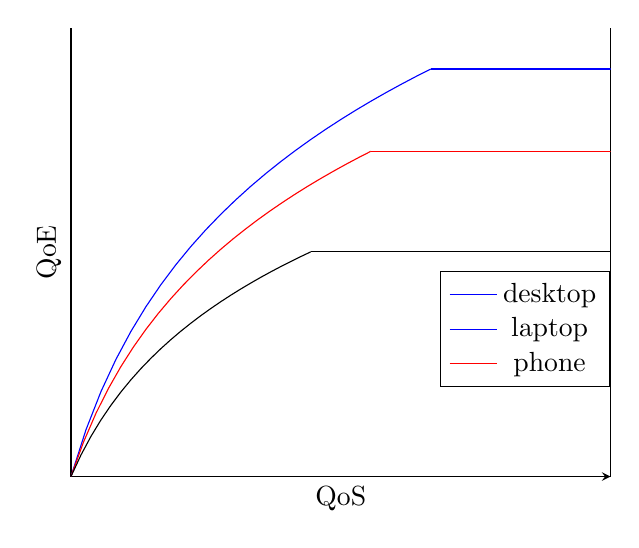
\begin{tikzpicture}
        \begin{axis}[
            xlabel=QoS,
            ylabel=QoE,
            xmin=1,
            xmax=10,
            ymin=0,
            x axis line style={->},
            ticks=none,
            major x tick style = {opacity=1},
            minor tick length=0pt,
            axis x line=bottom,
            legend style={at={(1,0.20)}, anchor=south east,legend columns=1},
            ]

            \addplot+[domain=1:7,mark=none, color=blue]{1.5*ln(x)};
            \addplot+[mark=none, color=blue] coordinates {
                (7,2.919)
                (10,2.919)
            };
            \addlegendentry{desktop}

            \addplot+[domain=1:6,mark=none, color=red]{1.3*ln(x)};
            \addplot+[mark=none, color=red] coordinates {
                (6,2.329)
                (10,2.329)
            };
            \addlegendentry{laptop}

            \addplot+[domain=1:5,mark=none, color=black]{ln(x)};
            \addplot+[style=solid, mark=none, color=black] coordinates {
                (5,1.609)
                (10,1.609)
            };
            \addlegendentry{phone}

        \end{axis}
    \end{tikzpicture}
    \caption{QoE as a function of QoS for different devices}
    \label{fig:utility}
\end{figure}


\section{Structure and Methodology}

Before trying to solve the problem we'll first evaluate the current video conferencing landscape in \autoref{chp:background}, to get a sense of the status quo. To limit the scope of what we're trying to accomplish, I'll define some test cases in \autoref{chp:test-cases} that we'll use throughout the thesis. We'll also evaluate one of the providers on the market today in \autoref{chp:experiments} by putting it to the test, running all the test cases from \autoref{chp:test-cases} to see how the service performs. Knowing this benchmark helps us evaluate the potential for my solution, which we'll take a look at in \autoref{chp:suggested-solution}. We'll discuss how our solution can be implemented and its strengths and weaknesses in \autoref{chp:discussion}, before summarizing what we've learned in \autoref{chp:conclusions}.


\section{Contribution}

This thesis proposes an approach to modelling video conferences with known inter-node latencies and bandwidths as a flow network, and shows how an efficient routing for video can be derived from the model using linear programming. The method also demonstrates how performance can get a significant boost by adding extra nodes to the flow network acting as repeaters and transcoders, bridging the performance gap between traditional \gls{mcu}-backed solutions and peer-to-peer solutions.

I also benchmark the two most popular web browsers as of the time of writing, Google Chrome and Mozilla Firefox, in a set of test cases, and reveal severe flaws in how Firefox handles constrained nodes. Both browsers are shown to have lots of potential for increased performance. These tests were run with tools developed for this purpose, which are included in the appendices.


\section{Notation and Terminology}

Bandwidth will often be written like this: 10/5. That should be read as 10 Mbps download and 5 Mbps upload, unless another unit is specified.

A video conference will often be called a conversation in this thesis. The term ``video conferencing'' carries a lot of luggage from its early history, when the technology was cumbersome, expensive, and only applicable in business scenarios. The movement WebRTC represents is about the opposite, commoditizing the technology to make it cheap and accessible to everyone, allowing it to enter the private domain. Friends don't ``confer'' between themselves; they converse. Names say a lot about a technology's intended application, thus if we want the technology to enter the private domain we need a name for it that does not convey business usage. Hence the term used in this thesis: video conversations. The even less formal ``video chat'' could also have fit the bill, but that feels like it leaves the business side entirely in the dark; conversation feels like a good middle ground that is applicable to both sides.


\section{Disclaimer}

This thesis does not try to measure or solve for audio transmission, as that's a much simpler problem that can practically always be completed by sending the same stream to all nodes in the conversation. There's always only one stream to encode, it doesn't noticeably affect available bandwidth, and it's already widely deployed. However, results we achieve for video can also be applied to audio streams if the environment is very heavily constrained or further optimization is required, but is out of scope for this thesis.
